\section{Approach}\label{s:approach}

In order to enforce reservations while still running best effort jobs
opportunistically, our approach is use priority scheduling.

We describe how priority scheduling solves the enforcement problem that weights
has, as well as its dependence on hardware ticks
(\autoref{ss:approach:solves-problems}). Linux has priority scheduling for real
time applications (\autoref{ss:approach:linux-classes-isolate}), but they are
not a good fit for microservice workloads
(\autoref{ss:approach:linux-classes-bad-fit}).

\subsection{Priority scheduling solves the problems with
weights}\label{ss:approach:solves-problems}

Enforcing global prioritization between two priorities is simpler and requires
fewer global runqueue searches, where cores have to look at all the others'
runqueues, than enforcing a weight split does. 

It is simpler because priorities are: a core does not need to do complex
accounting to figure out whether it is a low-weight processes turn to run, it
just needs to know the set of runnable priorities. Enforcing the global
prioritization between them equivalent to choosing only from the highest
priority.

Enforcing priorities also requires fewer global runqueue searches, because they
only need to happen on \textit{class boundary crossings}: on \exit{}, when a
core switches to running lower class processes after having previously been
running high class, and on \entry{}, when a core enqueues a higher class
process. These checks ensure that if a core $c$ is currently running a BE thread
$t$, the scheduler knows that there are no queued and waiting LC threads
anywhere on the machine. If there is a queued LC thread on a different core $c'$
when $c$ starts running $t$, the \exit{} check, that looks at every cores'
runqueue, will see and steal it. If a new LC thread wakes up on a different core
while $t$ is running, the \entry{} check ensures that $c'$ will look at $c$'s
runqueue, see that it is running a BE thread, and will send the new LC thread to
$c$ via an interrupt, where the interrupt handler will trigger a scheduling that
interrupts $t$.

Strict priorities being enforced at class boundary crossings also means that how
quickly a runnable LC process gets access to a core it reserved (not already
running one of its threads) is now dependent on how quickly the handler for
process wakeup or dequeue runs, which in Linux is on the order of a few
microseconds. Currently it is on the order of however often the load balancer
runs (which is a complicated number that is dependent on how close the two cores
are in the CPU architecture hierarchy, as well as how loaded the machine is),
and even in a scheme where weight was enforced globally it would be on the order
of a scheduling tick (4ms). For enforcing sharing across long-running processes
balancing occasionally works well, but for workloads with runtimes on the order
of low to mid double-digit ms, those delays significiantly influence final
processing times.


\subsection{Linux scheduling classes enforce
priorities}\label{ss:approach:linux-classes-isolate}

Linux already provides priority scheduling across scheduling classes, of which
it has three that are accessible to users (in descending order of priority):
\deadlineclass{}, \rtclass{}, and \normalclass{}. Generally speaking most load
is expected to fall into the \normalclass{} scheduling class (hence the name).
It is the default scheduling class, and both latency critical and best effort
processes run in it. It is only within the \normalclass{} scheduling class that
the \cgroups{} cpu.weight interface is relevant.

Each scheduling class exists completely separately: classes maintain their own
runqueues and per-entity state; implement their own scheduling algorithms to
choose from the entities on their runqueue; and balance the load across
runqueues on different cores. 

Linux prioritizes strictly between different scheduling classes: it only
schedules a lower scheduling class if the higher scheduling classes found
nothing to run, and each scheduling class tries to steal work from other cores
before returning that it has nothing to run.

\begin{figure}[t]
    \centering
    \begin{subfigure}[t]{\columnwidth}
        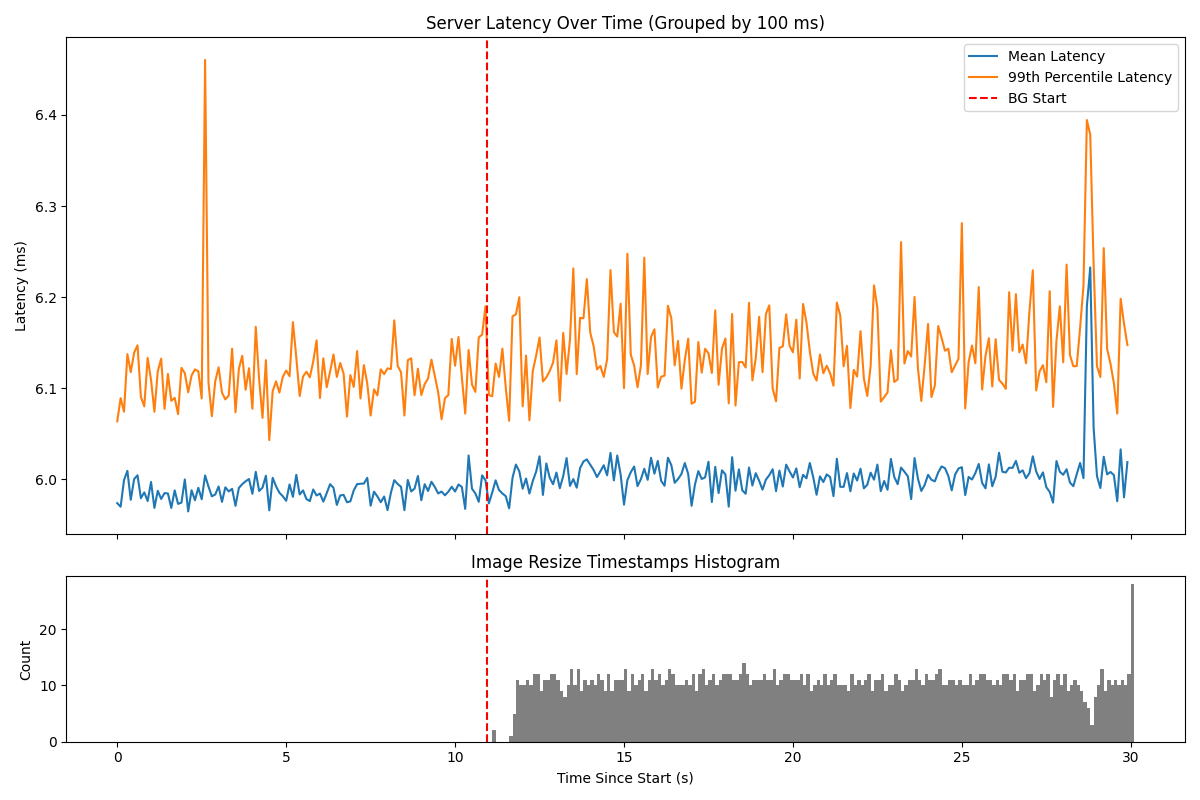
\includegraphics[width=\columnwidth]{graphs/srv-bg-rt-low.png}
        \caption{Low load (85\%)}\label{fig:srv-bg-rt-low}
        \vspace{12pt}
    \end{subfigure}
    \hspace{\fill}
    \begin{subfigure}[t]{\columnwidth}
        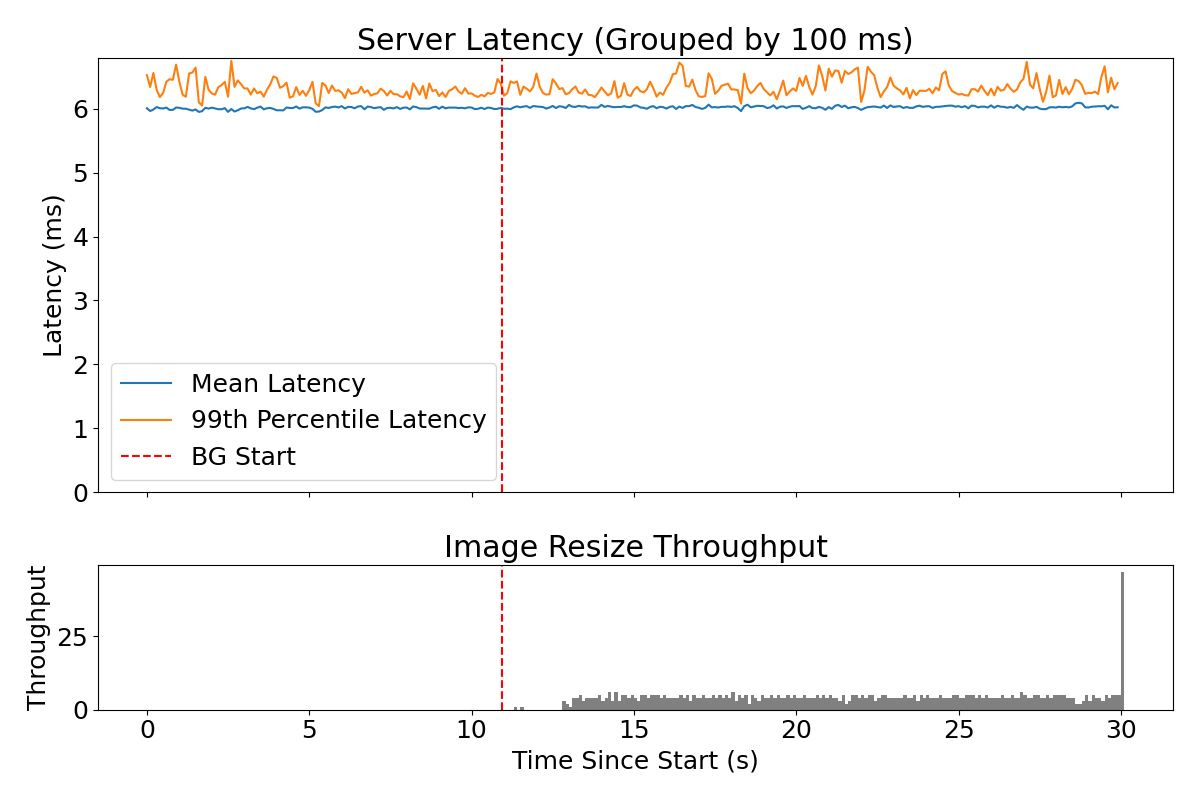
\includegraphics[width=\columnwidth]{graphs/srv-bg-rt-high.png}
        \caption{High load (95\%)}\label{fig:srv-bg-rt-high}
    \end{subfigure}
    \vspace{4pt}
    \caption{when running the server as a real time application, Linux does a
     good job of isolating the server's latencies from the load from best effort
     jobs }\label{fig:srv-bg-rt}
\end{figure}

\autoref{fig:srv-bg-rt} shows the result of running the same microbenchmark from
\autoref{fig:srv-bg-weight-150}, but with the LC server running in the
\rtclass{} scheduling class. We can see that in both load settings the tail and
average latency stays stable at $\sim$6.0ms after starting the BE workload. The
throughput of the image resize job (10 iter/100ms at low load, and 5iter at high
load) is around 80\% of what it was in \autoref{fig:srv-bg-weight-150} when
running the server with \cgroups{} weights.

\subsection{Linux scheduling classes are not suited to enforce microservice
reservations}\label{ss:approach:linux-classes-bad-fit}

We conclude a possible alternative to using \cgroups{}: run latency critical
applications that have reservations in the real time \rtclass{} scheduling
class, and best effort ones in \normalclass{}.\footnote{The \deadlineclass{}
scheduling class is not a good fit, since it requires accurate knowledge of a
processes runtime (processing time per request) and period (when requests come
in)} However, we show that the schedulers within each priority are not suited
for microservices (\autoref{sss:approch:linux:policies}), and that Linux method
of avoiding starvation has adverse effects on the LC application
(\autoref{sss:approach:linux:starve-throttle}).

\subsubsection{Real time schedulers are unsuitable for microservice
workloads}\label{sss:approch:linux:policies}

Running a microservice in \rtclass{} is untenable because of \rtclass{}'s
intra-priority schedulers. \rtclass{} has two different scheduling policies:
\schedfifo{} and \schedrr{}. Both have 99 priorities between which they enforce
strict priority; within priorities they differ in the policy they enforce.

\schedfifo{} uses first-in-first-out run-to-completion scheduling. This means
that within each class, the process to run next will be the one that woke up
first, and it will run until it blocks or exits. When a blocked thread becomes
runnable again, that is counted as a wakeup and it will be put on the back of
the queue. This is known to have a failure mode of head-of-line (HoL) blocking
under varied request processing times, where long-running requests monopolize
the CPU while short requests wait in the queue.

\schedrr{} addresses this concern by running a round-robin scheduler that will
ensure Processor Sharing within each priority. Every thread just gets the same
scheduling quantum and then gets put at the end of that priority's queue. This
means that within each priority CPU time is allocated based on the number of
runnable threads. This conflicts with how weights are used within runqueues to
allocate CPU time between different LC workloads. Kubernetes, for instance,
allows users to make fractional CPU requests, which are enforced using
weights.\hmng{next part is just conjecture, should I just leave it out?}
Similarly, a provider might overprovision vCPUs of tenants VMs to actual
hardware cores. We can't know what they use to configure access to the
underlying cores, but we know they use \cgroups{} to do so for serverless
functions because that's what Firecracker uses~\cite{firecracker-cgroups}.
Although \cgroups{} limits (\ie{} defining a maximum amount of runtime per
period each group can get) can also be applied to cgroups in real time
applications, both of these use cases require the weight interface to ensure the
split they want. In Kubernetes, this is required for Burstable containers \hmng{
not clear why it's needed in the VM setting? }

\subsubsection{Linux throttles \rtclass{} processes under high load
}\label{sss:approach:linux:starve-throttle}

Schedulers running priority scheduling have to contend with the possibility of
starvation. Starvation can have many negative effects: it can cause deadlocks if
a low and high priority process share a lock (either in user-space or in
kernel-space), TCP connections can die while the process is being starved, and
it can miss interrupts like timers or completed i/o requests.

To avoid these, Linux chooses to carefully ensure that no process is ever
starved, which it does by throttling high class processes with high load. Linux
has two different safeguards that enforce that no process is ever starved. One
is that \rtclass{} is as a scheduling class rate-limited: there are tuneable
parameters \texttt{sched\_rt\_runtime} and \texttt{sched\_rt\_period}, that
together define a rate limit for the \rtclass{} as a whole. The other safegaurd
is that, even when set to be equal (\ie{} \rtclass{} gets the full runtime each
period if it wants), the \normalclass{} scheduling class also has a so-called
\textit{deadline server}, which ensures it gets a small amount of time. The
deadline server is a `process' is in the \deadlineclass{} scheduling class with
a small amount of runtime per period, then when chosen will pass control on to
the \normalclass{} scheduler~\cite{lkml-deadline-srv}.

The throttling Linux chooses to do interferes with the goal of honoring
reservations, because it throttles the LC experiencing high load, which is
precisly when it needs its full reservation  most.


\begin{figure}[t]
    \centering
    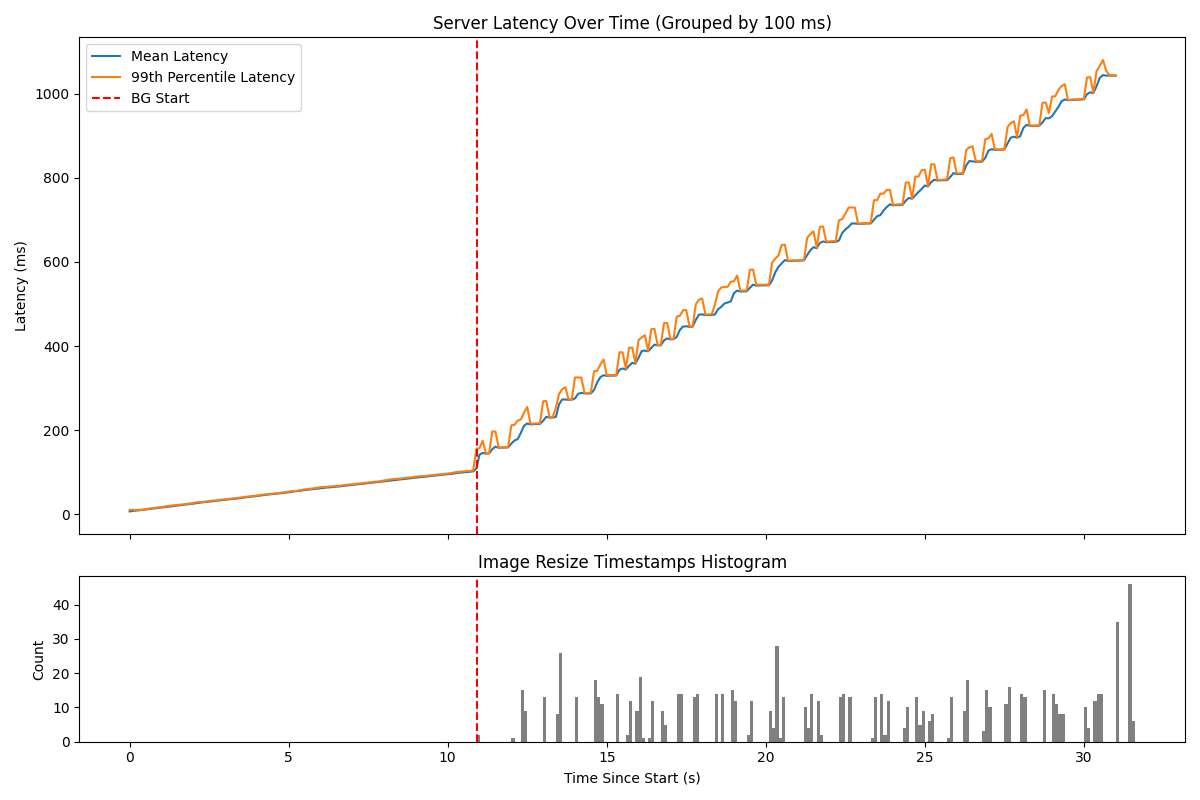
\includegraphics[width=\columnwidth]{graphs/overload-rt.png}
    \caption{LC in real time, throttling}\label{fig:overload-rt}
\end{figure}



Doing so impacts the performance of processes in the \rtclass{} at high load. We
can see this happen when we run the same microbenchmark experiment at a much
higher baseline utilization ($\sim$ 100\%). The results are in
\autoref{fig:overload-rt}. We see spikes begin to appear after starting the
image resize job, as the \rtclass{} server gets throttled in favor of running
the BE task; we see parallel spikes in the BE's throughput in the bottom graph.
Notice also the increase of the slope of response times after starting the
background tasks, this happens as the client has to queue requests while all the
current connections are blocked on running requests.

We conclude that Linux's mechanism of scheduling classes can enforce
reservations effectively, but that existing scheduling classes use algorithms
that are not a good fit for modern workloads, and that Linux throttles high
priority classes under high load.
